\begin{titlepage}
\title{\Huge{\textbf{Un Compilatore a Oggetti per Kitten}}}
\author{{\Large{\textbf{Fausto Spoto}}}\\{\normalsize\textit{Dipartimento di Informatica}}\\{\normalsize\textit{Universit\`a di Verona}}}
\end{titlepage}
\date{\vspace*{10ex}\begin{center}
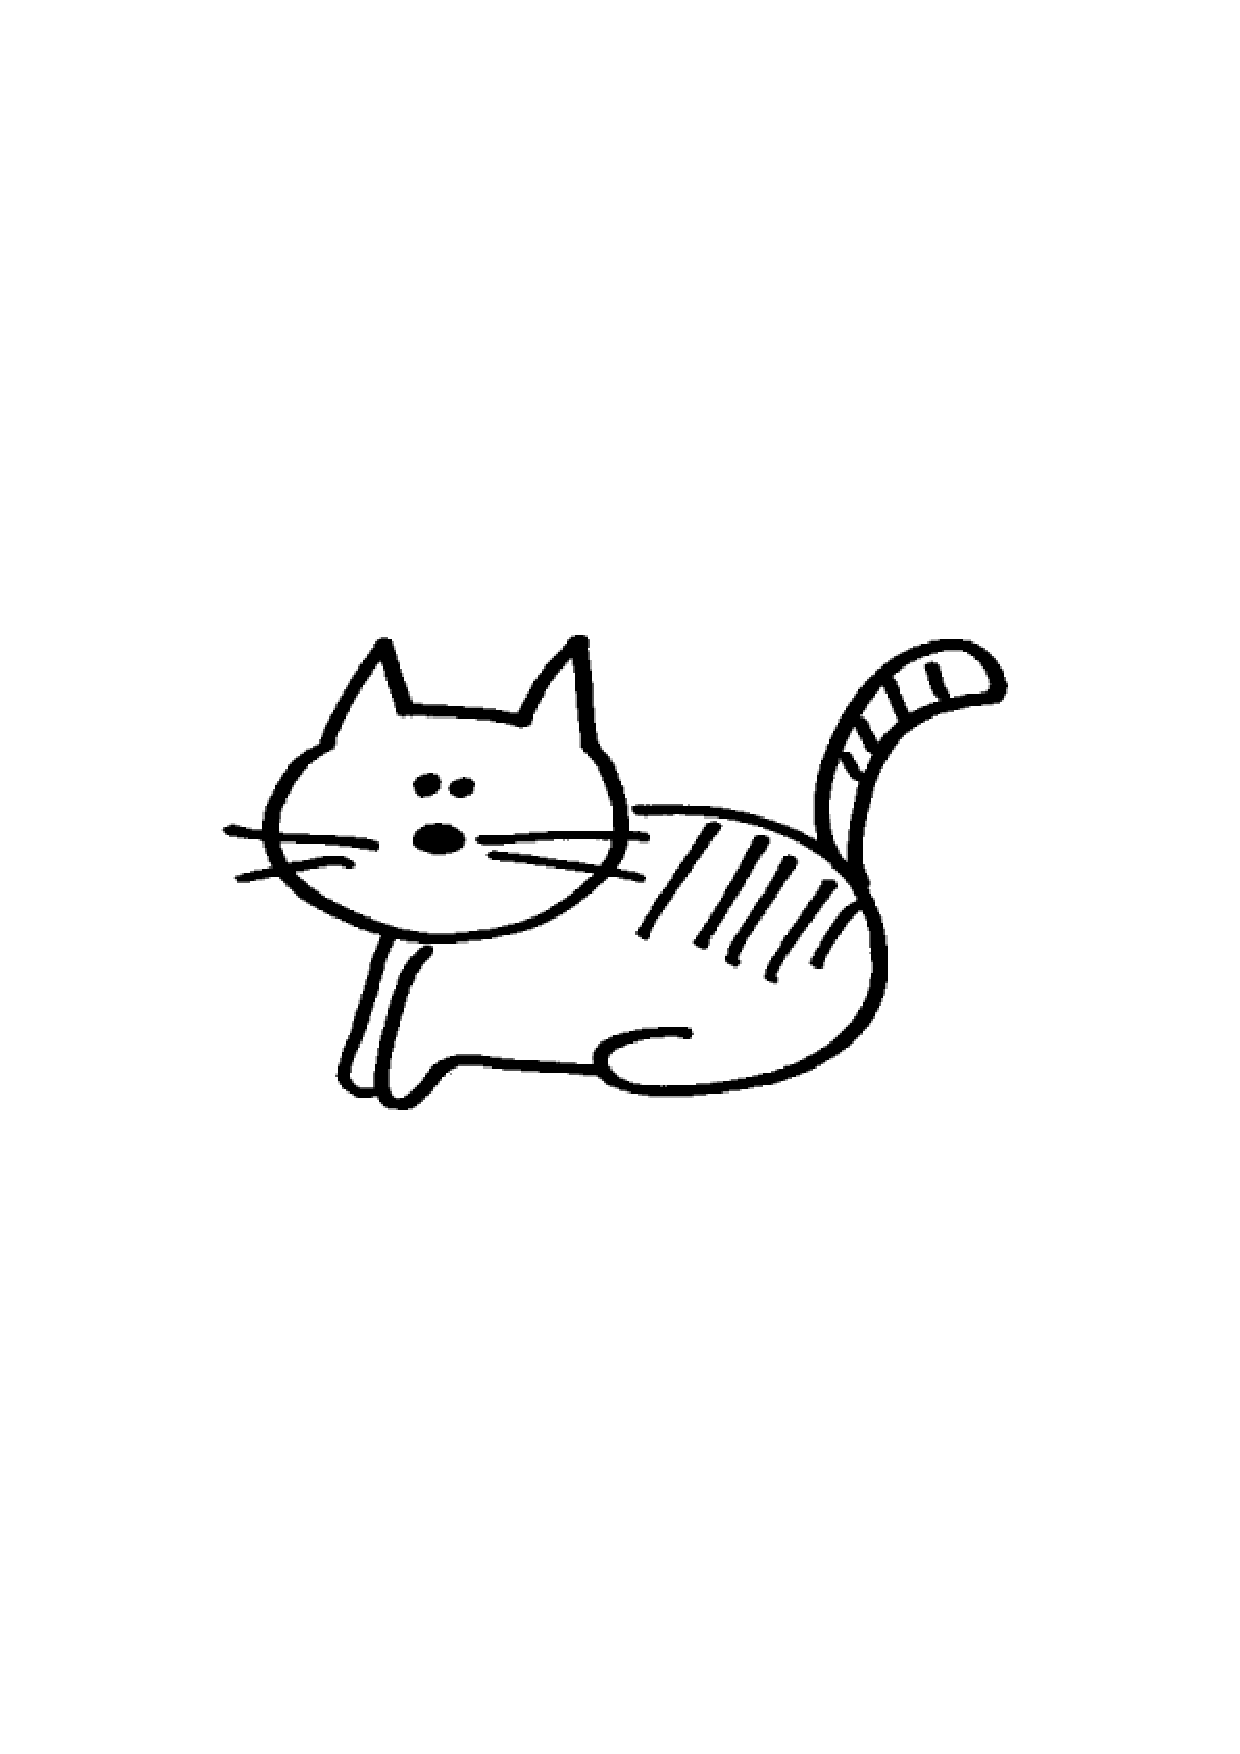
\includegraphics[width=7cm]{cat1.pdf}
\end{center}
}

\maketitle


%%%%%%%%%%%%%%%%%%%%%%%%%%%%%%%%%%%%%%%%%%%%%%%%%%%%%%%%%%%%%%%%%%%%%%%%%%%%%%%
%   Dedication Page                                                           %
%%%%%%%%%%%%%%%%%%%%%%%%%%%%%%%%%%%%%%%%%%%%%%%%%%%%%%%%%%%%%%%%%%%%%%%%%%%%%%%
\thispagestyle{empty}
\newenvironment{dedication}
  {\cleardoublepage \thispagestyle{empty} \vspace*{\stretch{1}} \begin{center} \em}
  {\end{center} \vspace*{\stretch{3}} \clearpage}

%\begin{dedication}
%A Futamura.
%\end{dedication}
% \cleardoublepage generates one blank page for the next 'Abstract'
% to be on an odd page.
%\thispagestyle{empty} \cleardoublepage

%%%%%%%%%%%%%%%%%%%%%%%%%%%%%%%%%%%%%%%%%%%%%%%%%%%%%%%%%%%%%%%%%%%%%%%%%%%%%%%
%   Abstracts                                                                 %
%%%%%%%%%%%%%%%%%%%%%%%%%%%%%%%%%%%%%%%%%%%%%%%%%%%%%%%%%%%%%%%%%%%%%%%%%%%%%%%

\mbox{}\\
\newpage
\pagenumbering{roman} \setcounter{page}{1}
\chapter*{Presentazione\markboth{Presentazione}{Presentazione}}

Scrivere un nuovo libro per un corso di compilazione sembra
un'operazione persa in partenza. \`E da venti anni che il
\emph{dragon book} di Aho, Sethi e Ullman~\cite{AhoSU86}
rimane sul mercato come
l'unico e insostituibile riferimento per chi si cimenta nella rara
e tuttora difficile arte di scrivere un compilatore. Ma gli anni passano
ed ecco che da una parte i corsi di laurea relegano la compilazione
nello spazio di poche lezioni; dall'altra l'evoluzione tecnologica dei
linguaggi di programmazione rende il \emph{dragon book} carente quanto
al trattamente della compilazione dei linguaggi \emph{a} oggetti
e della stessa compilazione \emph{con} gli oggetti. Perch\'e
la diffusione dei linguaggi a oggetti non \`e stata un cambiamento di
facciata per quanto riguarda il mondo dei compilatori: essa valorizza
il sistema di tipaggio del linguaggio; richiede
di spostare a tempo di esecuzione controlli e legami altrimenti
effettuati a tempo di compilazione; rende desiderabili nuove tecniche
di analisi e ottimizzazione del codice; infine, la stessa
implementazione a oggetti di un compilatore
rende pi\`u credibile la sua correttezza e permette l'implementazione
di ottimizzazioni tramite specializzazioni di classi e metodi della
sintassi astratta. Un limite del dragon book rimane
infine l'assenza di una trattazione della generazione di codice effettivamente
eseguibile, il che lascia lo studente di fronte a una storia interrotta,
senza la possibilit\`a di giocare col risultato della compilazione.

Ecco quindi nascere la necessit\`a di questo libro sulla
compilazione a oggetti di un linguaggio a oggetti. Non mancano certo
altri tentativi in questa direzione. Fra i tanti, non possiamo dimentivare
il libro di Appel~\cite{Appel02},
che ha inizialmente ispirato questo testo, specialmente per gli
esempi di analisi sintattica. Ma le
nostre soluzioni per il tipaggio statico e la generazione del codice
non sono assolutamente assimilabili alle tecniche dell'Appel, scarsamente a oggetti.
Inoltre in questo testo si arriva alla generazione di codice effettivamente
eseguibile in formato Java bytecode, il che rende l'utilizzo e la modifica
del compilatore \piu interessante per gli studenti.

Questo libro si offre come supporto allo studente impegnato in un corso
di compilazione che a Verona \`e organizzato in appena
una quarantina di ore
di lezione, laboratorio incluso. Le scelte
che hanno guidato la selezione degli argomenti trattati sono quelle
dell'utilizzo intensivo della programmazione a oggetti; dell'evidenziazione
continua della relazione biunivoca fra teoria e implementazione di
un compilatore; della maggiore
importanza data alle fasi avanzate della compilazione,
come controllo dei tipi e generazione del codice,
rispetto alle prime fasi di analisi lessicale e sintattica.

Un ringraziamento va agli studenti che hanno seguito a Verona
il mio corso di compilazione negli ultimi anni. \`E dall'interazione
che ho avuto con loro che deriva la presentazione degli argomenti trattati
in questo libro. Sono loro e i loro dubbi che mi hanno spinto a
scrivere un libro e del codice che fosse
facilmente comprensibile e meno ambiguo possibile.
La scarsa presenza di bug nel compilatore Kitten \`e il risultato
della loro, spesso involontaria, verifica.

{\flushright Fausto Spoto\\\hfill Verona, gennaio 2007}

\mbox{}\\

La revisione di questo testo e del compilatore Kitten ha comportanto una
semplificazione del codice e della sua presentazione, nonch\'e
la sostituzione dei makefile con dei task Ant. Il risultato sono
un compilatore Kitten e un libro pi\`u semplici e accessibili per
gli studenti.

{\flushright Fausto Spoto\\\hfill Verona, aprile 2015}

%%%%%%%%%%%%%%%%%%%%%%%%%%%%%%%%%%%%%%%%%%%%%%%%%%%%%%%%%%%%%%%%%%%%%%%%%%%%%%%
%   Acknowledgements                                                          %
%%%%%%%%%%%%%%%%%%%%%%%%%%%%%%%%%%%%%%%%%%%%%%%%%%%%%%%%%%%%%%%%%%%%%%%%%%%%%%%
%\chapter*{Acknowledgements\markboth{Acknowledgements}{Acknowledgements}}
%Your acknowledgement goes here...

%%%%%%%%%%%%%%%%%%%%%%%%%%%%%%%%%%%%%%%%%%%%%%%%%%%%%%%%%%%%%%%%%%%%%%%%%%%%%%%
%   Contents and Lists                                                        %
%%%%%%%%%%%%%%%%%%%%%%%%%%%%%%%%%%%%%%%%%%%%%%%%%%%%%%%%%%%%%%%%%%%%%%%%%%%%%%%
\newpage
%\renewcommand{\contentsname}{Indice}  % Original name = Contents
\tableofcontents
\cleardoublepage

%%%%%%%%%%%%%%%%%%%%%%%%%%%%%%%%%%%%%%%%%%%%%%%%%%%%%%%%%%%%%%%%%%%%%%%%%%%%%%%
%   Arabic numbering after this                                               %
%%%%%%%%%%%%%%%%%%%%%%%%%%%%%%%%%%%%%%%%%%%%%%%%%%%%%%%%%%%%%%%%%%%%%%%%%%%%%%%
\pagenumbering{arabic} \setcounter{page}{1}

